\documentclass[a0paper,fleqn]{betterposter}
\usepackage{graphicx}
\usepackage[colorlinks=true]{hyperref}

\begin{document}	
\betterposter{
%%%%%%%% MAIN COLUMN

\maincolumn{
%%%% Main space

	\textbf{Are there geographical biases in the study of language variation and change?}


}{
%%%% Bottom space
	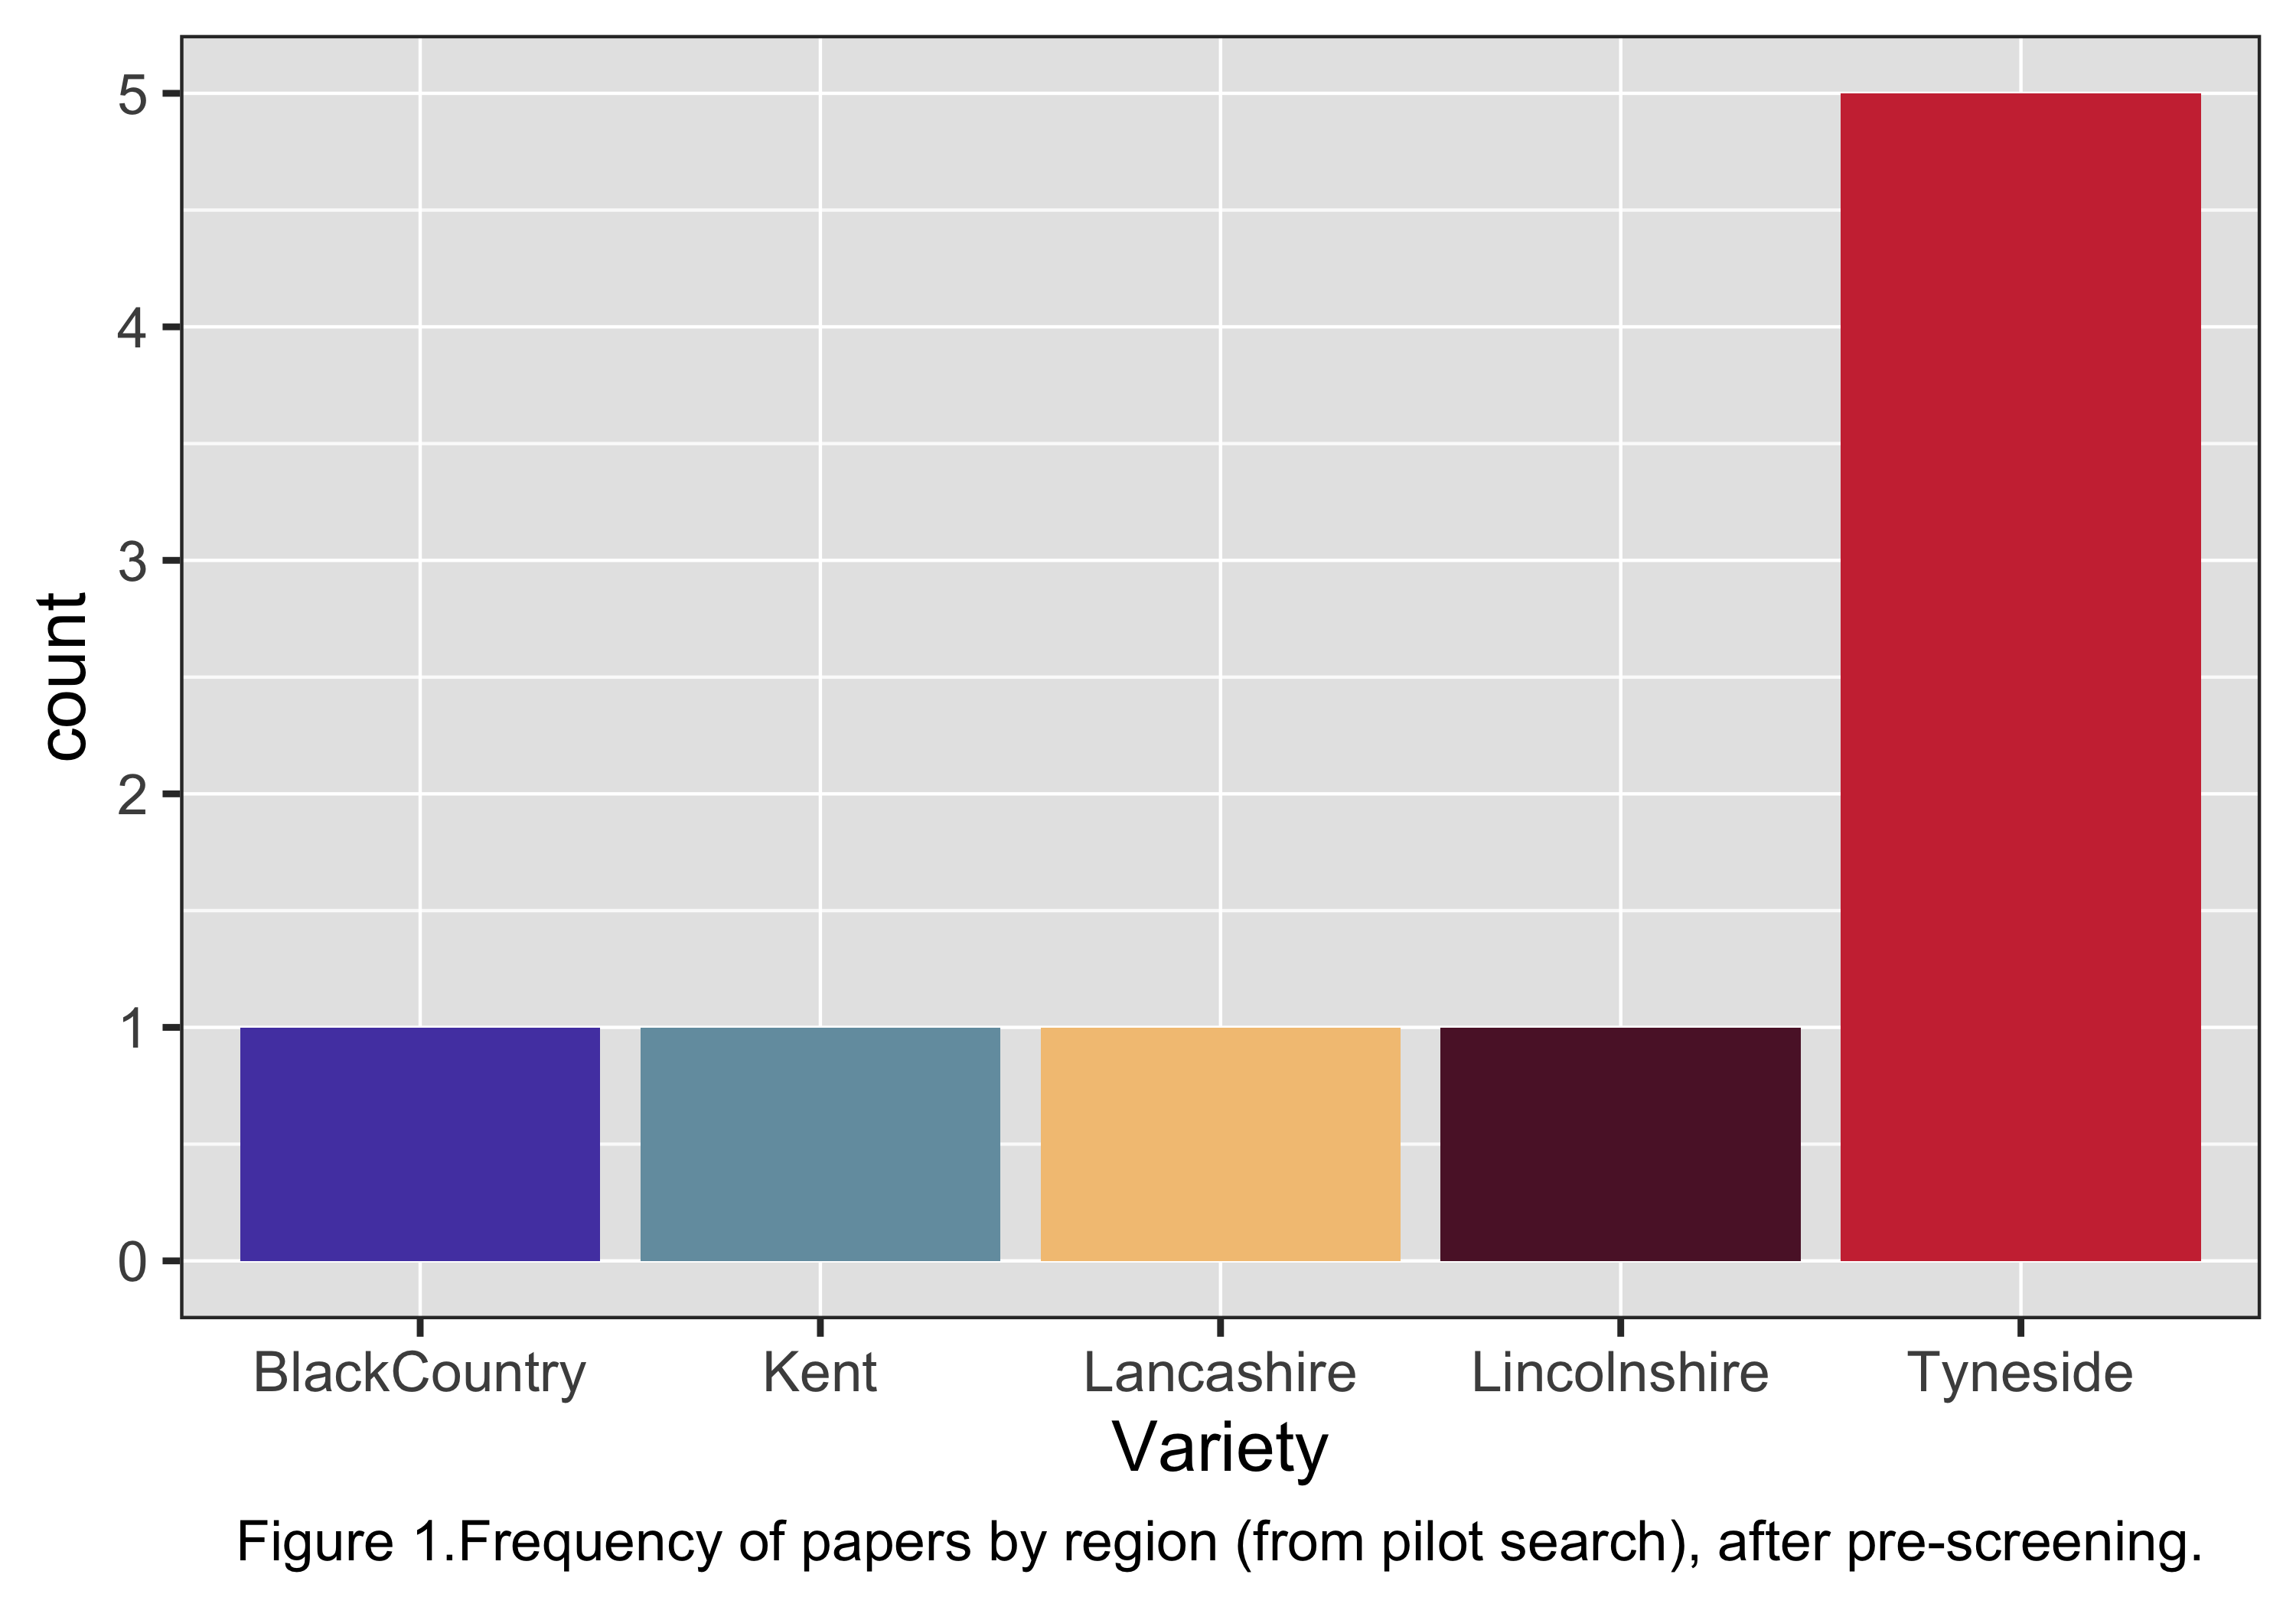
\includegraphics[scale=0.4]{posterPlot.png}
	\compactqrcode{frame-2.png}{Scan to access materials for this study on Github.}
}

}{
%%%%%%%% LEFT COLUMN

\title{Minority \\ Report}
\author{Caitlin Halfacre}
\author{Liam Keeble}

\institution{Newcastle University}

\section{Introduction}

Bias in science is unavoidable, and sociolinguistics is no different. In order to combat sources of bias, we must first identify its existence. With this study we aim to assess:
\begin{itemize}
\item whether there is bias towards studying some varieties of English over others.
\item whether location in relation to a research institution affect frequency of study of a variety of English.
\item other possible geographical/research characteristics (e.g. the existence of corpora/average income of the area) that may affects the frequency of studies published.
\end{itemize}

\section{Methods}

In order to meet our aims we:
\begin{itemize}
	\item Systematically searched \href{https://app.webofknowledge.com}{Web of Science} for studies on each particular variety of native English as identified by \href{https://en.m.wikipedia.org/wiki/List_of_dialects_of_English}{Wikipedia}.
	\begin{itemize}
		\item Search Term: (WC=(Linguistics)  AND  ((ALL="name of variety")  AND  ((ALL=sociolinguist*)  OR  (ALL=varia*)  OR  (ALL=change))))
		\item Document Type: All
		\item Timespan: 1982-2019 
	\end{itemize}
\end{itemize}
}
{
%%%%%%%%%Right column
	\section{Methods cont.}	
\begin{itemize}
%	\item Wikipedia was used as it serves as a kind of public self-identifier for speakers of speaking different varieties.
	\item pre-screened the resulting list and removed based on the inclusion criteria:
	\begin{itemize}
		\item the study assesses language variation or change
		\item study assesses the variety of English specified in the search
	\end{itemize}
	\item The remaining studies from each search were counted and the frequency of papers found per variety calculated.

\end{itemize}



\section{Pilot results}

For pilot data, we randomly sampled 10 varieties of English from all varieties found on the aforementioned wikipedia page, and searched for studies of language change in these varieties. These varieties were `Black Country', `Kent', `Lancashire', `Lincolnshire', `Tyneside', `Cornwall', `Suffolk', `Norfolk', `Northumbrian', `Staffordshire'.

\vspace{1cm}

\textbf{Table 1}. Poisson glm with area income and corpus existence as predictors of study frequency on a variety.

\begin{tabular}{ c c c }
	& Estimate & stand. error\\
	\hline
	Intercept & 4.25 & 2.52	\\
	Area income & -0.14 & 0.09\\
	Corpus? & 0.39 & 1.35 \\
\hline
\end{tabular}

\section{Questions from the pilot}
\begin{itemize}
	\item How do we narrow down the search terms?
	\item What do we do about edge cases such as studies of change using anecdotal data?
\end{itemize}



}


\end{document}



